\section{Mixing Messages and Transactions}
\label{section:mixing}

\begin{figure}[H]
    \centering
    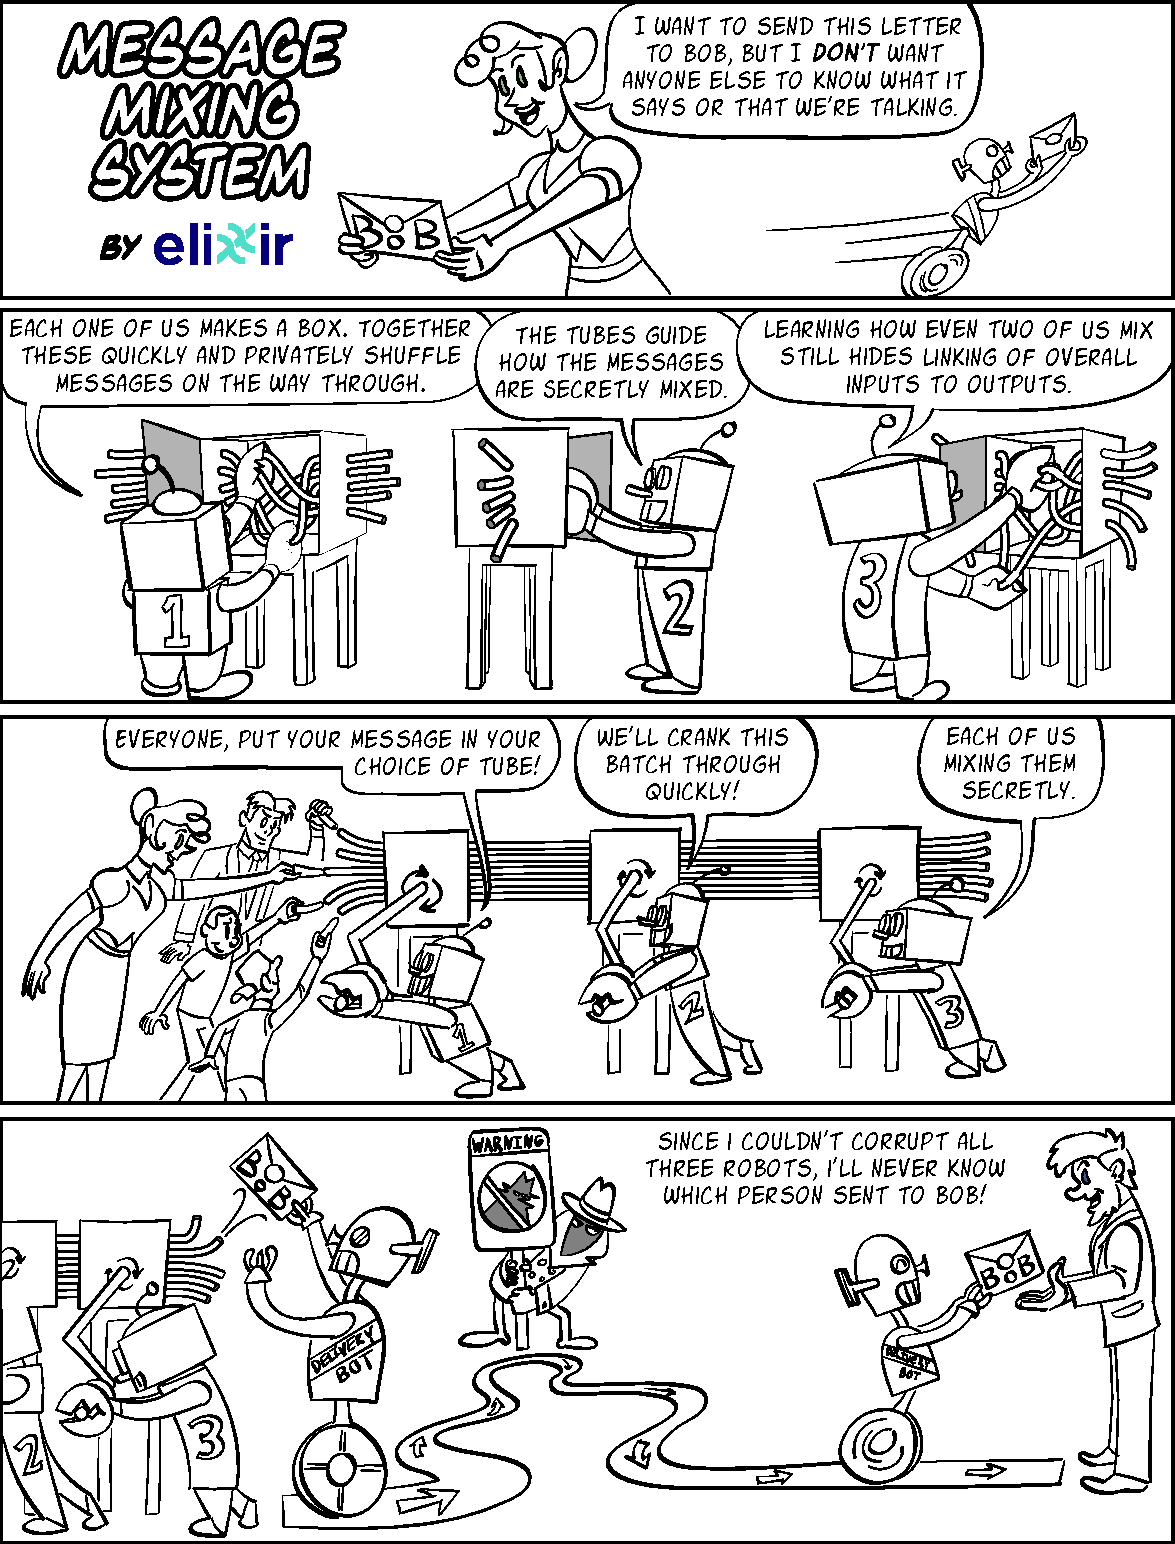
\includegraphics[width=\textwidth]{cartoons/MessageMixer.pdf}
    %\caption{Caption}
    %\label{fig:my_label}
\end{figure}

\break

Each team in the \name platform runs a single instance of a mixing network (mixnet) based on the cMix protocol~\cite{cMix}. Mixnets anonymize batches of messages and transactions, while protecting the confidentiality and integrity of each message. Besides supporting secure communications between users, these features are leveraged, and expanded to provide key functionality for the \name consensus protocol.
\iffalse
\begin{wrapfigure}{R}{0.75\textwidth}
    \centering
    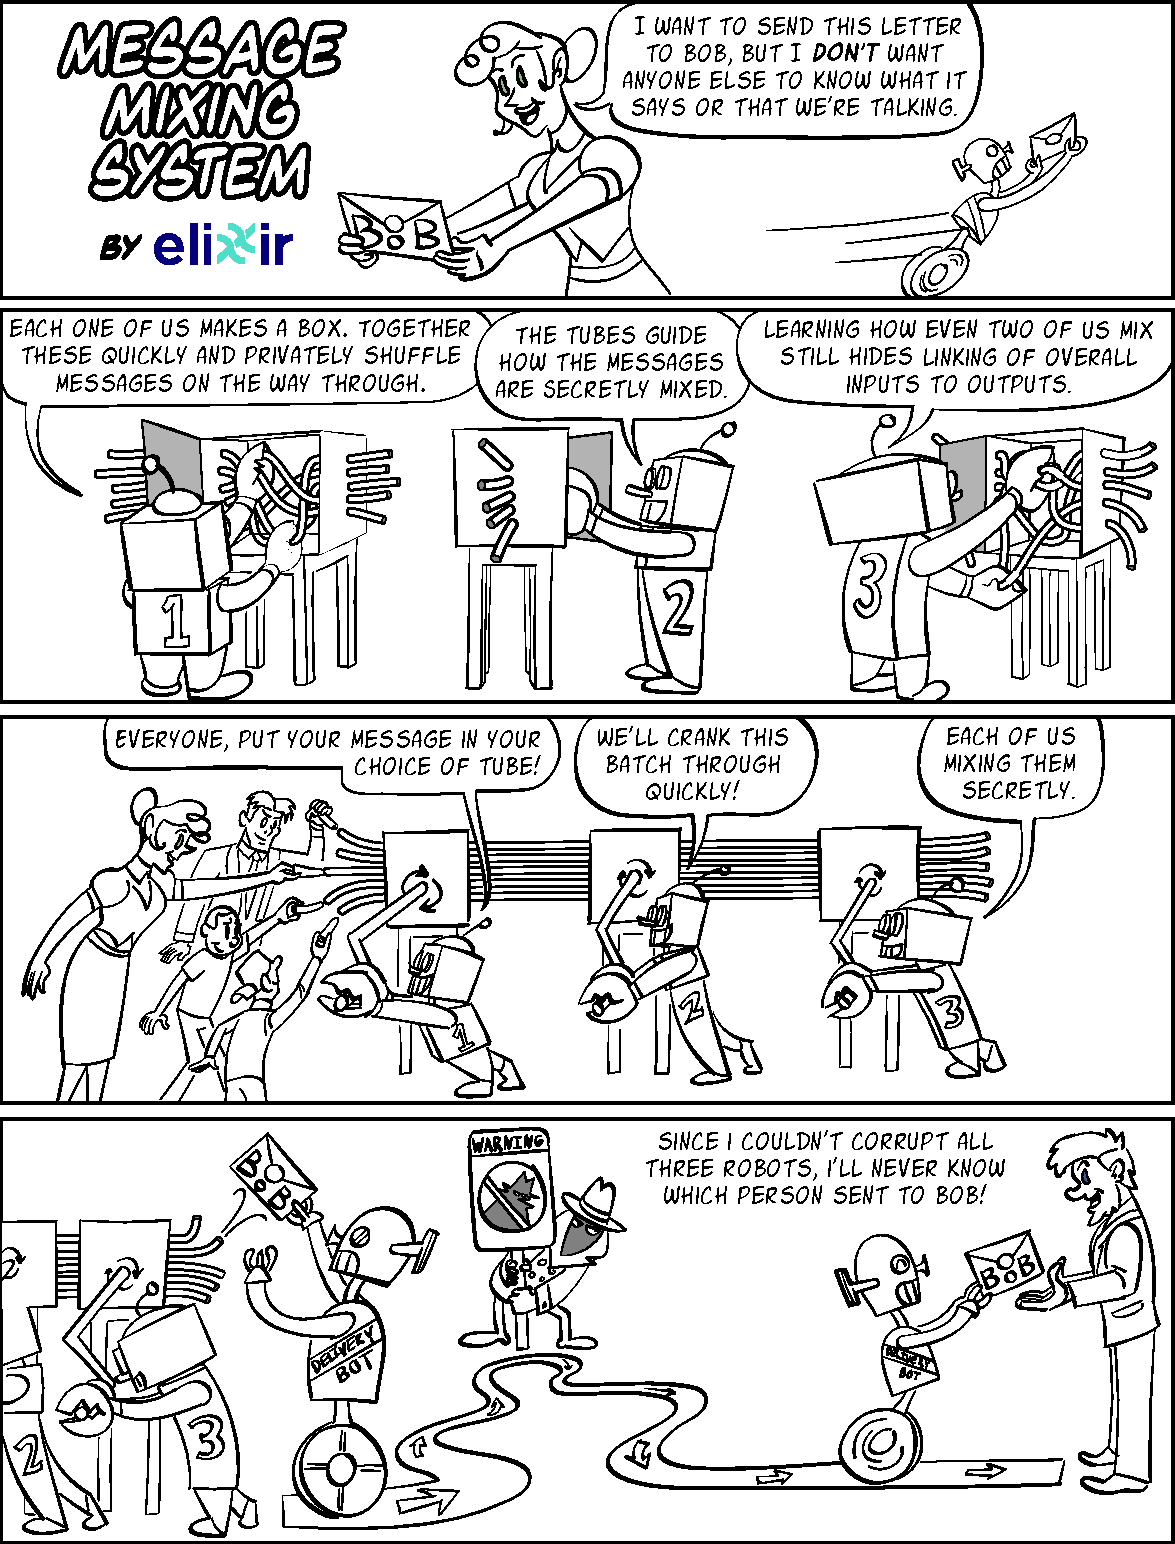
\includegraphics[width=0.74\textwidth]{cartoons/MessageMixer.png}
    %\caption{}
    %\label{}
\end{wrapfigure}
\fi

The cMix protocol is a breakthrough itself: it exhibits drastically lower real-time cryptographic latency than any other mixnet. By using a precomputation, the core cMix protocol eliminates all expensive real-time public-key operations performed on behalf of senders and recipients, and by nodes. This decreases real-time latency and lowers computational costs to clients. The core real-time phase, the second phase in the activity of a team, requires only a few quick computations, making it very well suited to applications running on lightweight clients, including chat messaging systems on smartphones, applications on low-power devices, and---most important---transaction processing.

Message processing in cMix involves 3 operations: Reception, Permutation, and Delivery. During Reception, masking network encryption is added to each already end-to-end encrypted message, while user-to-network encryption is removed from it, disassociating the senders identity from the message. In Permutation, the order of messages within a batch is shuffled, removing an observer's ability to correlate the order in which messages were received with the senders' identities. Finally, during Delivery, each node independently removes all masking network encryption, and sends the end-to-end encrypted message to its labeled destination.

The cMix Protocol has three additional important features that make it unique:

\begin{itemize}
    \item \textbf{Return Path}. The return path allows a receiver to send an immediate response through the mixnet; this permits receipts of transactions to be returned to users without the platform needing to know addressing information, thereby hiding the identity of the sender. To accomplish this goal, nodes generate additional keying material for the return path, and apply an inverse permutation so that responses arrive at the original senders.
    \item \textbf{Commitments}. Commitments are a protocol that produces data, often produced through hashing, that allows a third party to audit a computation performed by a node at a later date~\cite{commit}. All messages exchanged between nodes, the permutations they perform, and all keying materials in the mixnet's precomputation inherently function as commitments of how messages will be processed in the future, during the real-time phase of block generation. Nodes also produce a commit of the batch of encrypted messages before any decryption takes place. Commits function as an efficient mechanism for verifying that nodes perform their operations correctly.
    \item \textbf{Group Opening}. During the delivery operation, before each node in a team decrypts the batch of messages they have received, they create a commit of the batch, confirm with one another that all commits are identical, and then proceed to decrypt the batch independently. This guarantees that all nodes in the team work on the same content before any sensitive information is received. This prevents any single node from accessing sensitive information when other nodes are excluded from having the same access. This ensures that all honest nodes in the team are empowered to protect the integrity of the team and the properties they provide, namely confidentiality and anonymity.
\end{itemize}

With these features, \name provides integrity and anonymity for users sending messages and transactions through the platform. In \name, any honest node can, with non-negligible probability, identify nodes that violate integrity, and prevent malicious nodes improperly indicting an honest node. Lastly, any single honest node is able to protect user anonymity.